\chapter{Hiện thực và triển khai}

\section{Môi trường và công cụ phát triển}

Hệ thống được hiện thực thành nhiều thành phần chạy trong Docker Compose:
frontend Next.js, backend Python gRPC, các worker xử lý bất đồng bộ và các
dịch vụ hạ tầng gồm PostgreSQL, Redis, MinIO, Qdrant và Neo4j. Cách triển
khai này phù hợp cho môi trường phát triển, demo và staging; khi đưa vào
production có thể chuyển dần sang Kubernetes.

Các công cụ chính gồm:
\begin{itemize}
    \item \textbf{Next.js/TypeScript:} xây dựng giao diện người dùng và route
          LTI.
    \item \textbf{Python gRPC services:} hiện thực API và use case AI.
    \item \textbf{PostgreSQL, Qdrant, Neo4j, MinIO, Redis:} các thành phần lưu
          trữ và queue.
    \item \textbf{Docker Compose:} tái lập môi trường chạy local/staging.
    \item \textbf{LLM/Embedding provider:} sinh nội dung, embedding và hỗ trợ
          structured output.
\end{itemize}

\begin{figure}[H]
    \centering
    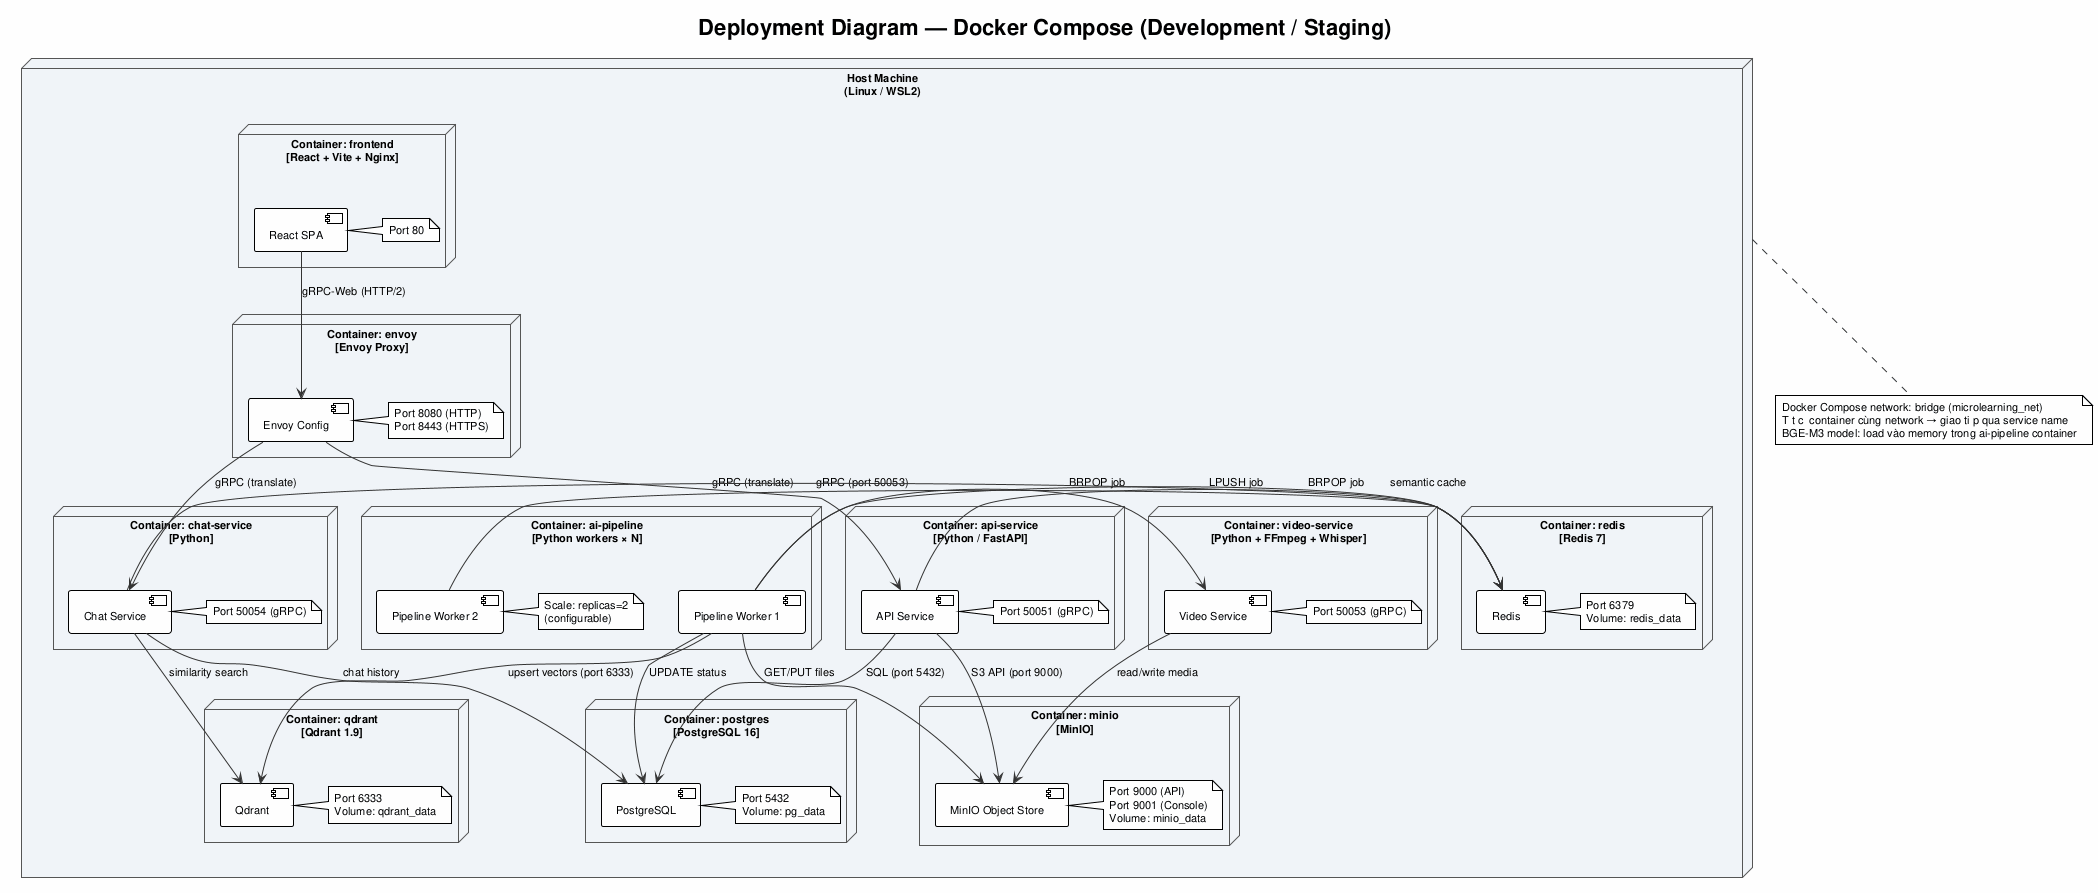
\includegraphics[width=0.95\textwidth]{diagrams/deployment_diagram.png}
    \caption{Deployment diagram của hệ thống.}
    \label{fig:deployment-implementation-lvtn}
\end{figure}

\section{Hiện thực Frontend và Backend}

\subsection{Next.js}

Frontend được xây dựng bằng Next.js và TypeScript. Thành phần này đảm nhận ba
vai trò chính:
\begin{itemize}
    \item Cung cấp giao diện giảng viên để upload, review và quản lý nội dung.
    \item Cung cấp giao diện học viên để xem card, làm quiz và nhận phản hồi.
    \item Xử lý LTI login/launch route để tích hợp với LMS.
\end{itemize}

Cấu trúc route chính:
\begin{itemize}
    \item \texttt{/lti/login}: khởi tạo OIDC login flow.
    \item \texttt{/lti/launch}: nhận LTI launch request và tạo session.
    \item \texttt{/manage/review}: màn hình giảng viên review nội dung AI.
    \item \texttt{/learn/cards}: màn hình học card.
    \item \texttt{/learn/quiz/[documentId]}: màn hình làm quiz theo tài liệu.
\end{itemize}

Session LTI được lưu phía server để giảm rủi ro lộ claim nhạy cảm trên client.
Frontend không tự quyết định quyền truy cập quan trọng mà dựa trên context đã
xác thực từ LTI/session và backend.

\subsection{Python gRPC Services}

Backend AI được hiện thực bằng Python, tổ chức theo Hexagonal Architecture.
Các use case chính nằm ở application layer, được gọi từ gRPC delivery hoặc
worker runner.

\begin{figure}[H]
    \centering
    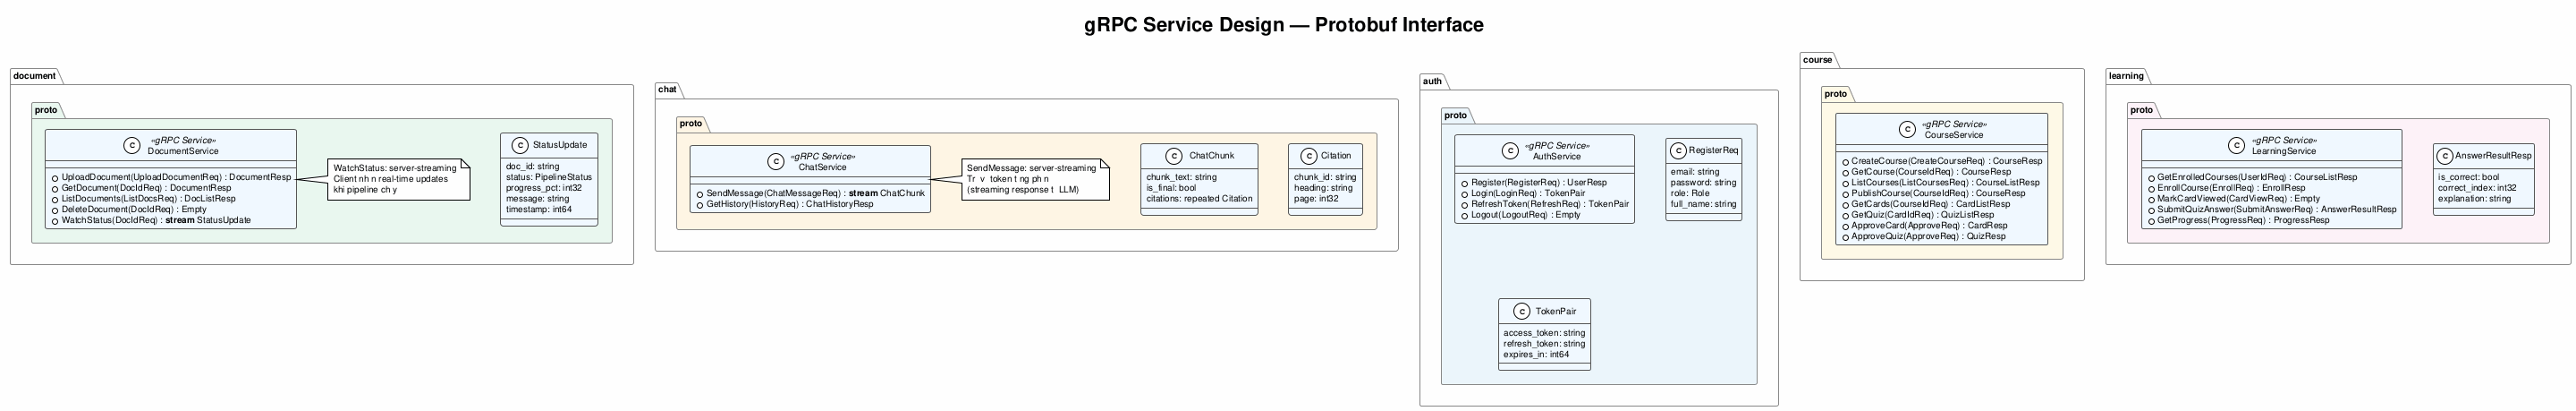
\includegraphics[width=0.95\textwidth]{diagrams/grpc_service_design.png}
    \caption{Hiện thực gRPC service và các use case tương ứng.}
    \label{fig:grpc-implementation-lvtn}
\end{figure}

Các nhóm API/use case chính:
\begin{itemize}
    \item \textbf{Document:} enqueue, process, delete, get status.
    \item \textbf{Search:} search chunks, search by learning outcome.
    \item \textbf{Generated content:} get cards, get quiz, generate curriculum
          quiz.
    \item \textbf{Curriculum:} ingest curriculum, list LO/chapter/assessment.
\end{itemize}

Dependency injection container khởi tạo adapter theo cấu hình môi trường. Khi
thiếu một dịch vụ hạ tầng trong môi trường test, hệ thống có thể dùng adapter
noop hoặc mock để kiểm thử use case.

\subsection{API Gateway}

API Gateway hoặc frontend server đóng vai trò cầu nối giữa UI, LTI session và
backend gRPC. Thành phần này kiểm tra session, chuyển đổi request từ giao diện
sang contract backend và mapping lỗi kỹ thuật thành thông báo dễ hiểu cho
người dùng. Với các endpoint cần streaming hoặc xử lý lâu, gateway chỉ khởi
tạo job và trả về trạng thái để frontend polling hoặc subscribe tiến trình.

\section{Hiện thực luồng xử lý bất đồng bộ}

\subsection{Workers}

Các worker giúp tách tác vụ nặng khỏi request/response trực tiếp:
\begin{itemize}
    \item \textbf{Document worker:} nhận job tài liệu, parse, chunk, embed và
          lưu metadata.
    \item \textbf{Enrichment worker:} sinh card/quiz bằng LLM và validate kết
          quả.
    \item \textbf{Outbox worker:} đọc sự kiện hoặc bảng outbox từ PostgreSQL
          để đồng bộ sang Neo4j.
\end{itemize}

Mô hình worker giúp frontend phản hồi nhanh sau khi upload, còn xử lý tài liệu
diễn ra bất đồng bộ. Khi lỗi tạm thời xảy ra, job có thể retry mà không yêu
cầu người dùng upload lại file.

\subsection{Queue}

Queue lưu các job xử lý tài liệu, embedding và generation. Mỗi job cần có
document ID, course context, số lần retry, trạng thái hiện tại và thông tin lỗi
cuối cùng. Worker cập nhật trạng thái để frontend hiển thị tiến trình cho
giảng viên.

\subsection{Embedding Jobs}

Embedding job nhận danh sách chunk đã được parse/chunk thành công. Worker gọi
embedding provider, chuẩn hóa vector và upsert vào Qdrant cùng metadata. Nếu
Qdrant hoặc provider tạm thời lỗi, job được retry có giới hạn; nếu hết retry,
document chuyển sang trạng thái lỗi để người dùng có thể xử lý lại.

\subsection{Quiz Generation Jobs}

Quiz generation job nhận context chunk, Learning Outcome, Bloom level và cấu
hình số lượng câu hỏi. Worker gọi LLM, validate structured output, lưu quiz
item, options, correct answer, explanation và source chunk. Kết quả được lưu ở
trạng thái draft để giảng viên review trước khi publish.

\section{Tích hợp LMS}

\subsection{Open edX}

Open edX là nền tảng tích hợp chính trong bản hiện tại. Hệ thống được nhúng
vào khóa học thông qua LTI 1.3. Khi học viên hoặc giảng viên mở activity từ
Open edX, LMS gửi LTI launch request đến frontend. Frontend xác thực request,
tạo session và điều hướng đến màn hình học hoặc quản lý.

Ưu điểm của Open edX là phù hợp môi trường đại học, hỗ trợ course context và
có cộng đồng triển khai lớn. Nhược điểm là vận hành tương đối nặng, đặc biệt
khi dùng Tutor stack đầy đủ.

\subsection{Moodle}

Moodle được phân tích như hướng triển khai tương thích. Moodle hỗ trợ LTI tốt
và nhẹ hơn Open edX trong một số môi trường. Vì hệ thống đóng vai trò LTI Tool
Provider, về nguyên tắc có thể đăng ký như external tool trong Moodle mà không
phải thay đổi lõi backend. Phần Moodle trong luận văn được xem là định hướng
mở rộng nếu chưa có demo end-to-end tương ứng.

\subsection{LTI Configuration}

Các thông tin cấu hình LTI gồm issuer, client ID, deployment ID, platform
JWKS/keyset URL, tool redirect URI và public/private key của tool. Các endpoint
xử lý LTI phải kiểm tra issuer, audience/client ID, deployment ID, nonce và
chữ ký JWT. Session cần có TTL hợp lý và không nên lưu claim không cần thiết ở
client.

\section{Đóng gói và triển khai}

\subsection{Docker Compose}

Docker Compose được dùng để triển khai local/staging. Các service chính gồm
frontend, backend gRPC, worker, PostgreSQL, Redis, MinIO, Qdrant và Neo4j.
Compose giúp tái lập môi trường demo nhanh, phù hợp với luận văn và quá trình
phát triển cá nhân.

\begin{lstlisting}[language=bash, caption={Ví dụ chạy stack triển khai local}]
docker compose up -d --build
\end{lstlisting}

\subsection{Deployment Architecture}

Kịch bản demo end-to-end dự kiến:
\begin{enumerate}
    \item Giảng viên đăng nhập hoặc mở tool từ LMS qua LTI.
    \item Giảng viên upload một tài liệu môn học.
    \item Hệ thống hiển thị trạng thái xử lý.
    \item Worker parse, chunk, embed và sinh card/quiz.
    \item Giảng viên review, sửa một số card/quiz và publish.
    \item Học viên mở bài học từ LMS, xem card và làm quiz.
    \item Hệ thống lưu kết quả và hiển thị phản hồi.
\end{enumerate}

Các thông tin nhạy cảm như LLM API key, database password, JWT/LTI secret và
private key phải được cấu hình qua biến môi trường hoặc secret manager. Trong
môi trường demo, có thể dùng file env cục bộ nhưng không commit giá trị thật
lên repository.

\subsection{Định hướng Kubernetes}

Kubernetes chưa được trình bày như triển khai production hoàn chỉnh. Hướng
chuyển đổi từ Docker Compose sang K8s gồm:
\begin{itemize}
    \item Mỗi service thành một Deployment hoặc StatefulSet phù hợp.
    \item PostgreSQL, Qdrant, Neo4j cần persistent volume.
    \item Secret quản lý LLM API key, LTI keypair và database password.
    \item Worker scale độc lập theo số lượng job.
    \item Ingress expose frontend và gRPC gateway nếu cần.
\end{itemize}

Phần này là định hướng triển khai, cần bổ sung manifest và kiểm thử vận hành
nếu luận văn yêu cầu production-grade deployment.
